\documentclass[10pt]{article}
\usepackage{geometry}
%\usepackage{showframe} %This line can be used to clearly show the new margins

\newgeometry{vmargin={25mm, 30mm}, hmargin={15mm,15mm}}   % set the margins

\usepackage{fancyhdr}

\pagestyle{fancyplain}

\usepackage{color}
\definecolor{headercolor}{rgb}{0.3922,0.5843,0.9294}

\usepackage{blindtext}%
\usepackage[theorems,breakable]{tcolorbox}%

\usepackage{tikz} % https://texample.net/tikz/examples/bisector/
\usetikzlibrary{calc,intersections}
\usepackage{tkz-euclide}

\fancypagestyle{cheader}{% https://tex.stackexchange.com/questions/69950/fancyhdr-color-and-width-of-line
	\fancyhf{}% Clear all headers/footers
	\fancyhead[L]{\raisebox{-.5\baselineskip}[0pt][0pt]{Mathematics}}% Header Centred
	\fancyhead[C]{\raisebox{-.5\baselineskip}[0pt][0pt]{\textbf{\Large Center}}}% Header Centred
	\fancyhead[R]{\raisebox{-.5\baselineskip}[0pt][0pt]{\today}}% Header Centred
	\fancyfoot[C]{-\hspace{5mm}\thepage\hspace{5mm}-}% Footer Centred
	\renewcommand{\headrulewidth}{2pt}% 2pt header rule
	\renewcommand{\headrule}{\hbox to\headwidth{%
			\color{headercolor}\leaders\hrule height \headrulewidth\hfill}}
	\renewcommand{\footrulewidth}{0pt}% No footer rule
}

\newtcbtheorem{problem}{Problem}{% https://tex.stackexchange.com/questions/198820/create-newshadetheorem-without-numbering
	theorem name,%
	colback=green!5,%
	colframe=green!35!black,%
	fonttitle=\bfseries,title after break={Problem  -- \raggedleft Continued}%
}{problem}

\newtcbtheorem{solution}{Solution}{%
	theorem name,%
	colback=green!5,%
	colframe=green!35!black,%
	fonttitle=\bfseries,title after break={Solution  -- \raggedleft Continued}%
}{solution}




\linespread{1.2}
\begin{document}
	\pagestyle{cheader}
	
	\begin{problem}{}{}
		
		\textit{Given an acute triangle $\triangle ABC$, construct with straightedge and compass square $DEFG$ 
		such that D and E are on $\overline{BC}$, G is on $\overline{AB}$ and F is on $\overline{AC}$.}
	\end{problem}

	\noindent
	Straightedge and compass can construct the middle point of a line segment, and perpendicular line 
	through a point on a line segment.
	
	\centering
	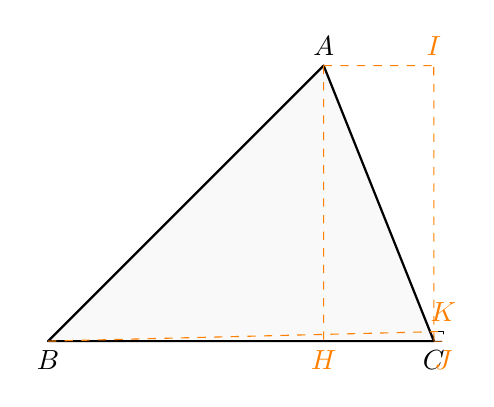
\begin{tikzpicture} [scale=0.7]
		%----------------------------------------------------
		% Coordinates of A, B and C, the triangle vertices 
		%----------------------------------------------------
		\tkzDefPoint (5, 5){A}
		\tkzDefPoint (0, 0){B}
		\tkzDefPoint (7, 0){C}
		\tkzLabelPoints[above](A)
		\tkzLabelPoints[below](B,C)
		\tkzDrawPolygon[thick,fill=gray!5](A,B,C);
		%\tkzDrawPoints(A,B,C)
		
		\tkzDefPointBy[projection = onto B--C](A) \tkzGetPoint{H};
		\draw [orange, dashed] (A) -- (H) node [right, below] {$H$};
		
		
		%\tkzDefLine(A, H) \tkzGetLength{height}
		
		%\tkzDefLine[orthogonal=through A](C,B)     
		%\tkzGetPoint{X_1}
		%  
		%\tkzInterLL(A,X_1)(B,C)
		%\tkzGetPoint{H5}
		%\draw [orange, dashed] (A) -- (H5) node [right, below] {$H$};
		%\tkzDrawPoints(H5)
		%\tkzDefLine(A, H) \tkzGetLength{height}
		%\tkzDefPoint (H5){H}
		
		%\tkzDrawAltitude[dashed,color=magenta](C,B)(A)   %% draw the perpendicular
		%\tkzGetPoint{P}                                  %% get the point P
		%\tkzLabelPoint[below](P){$P$}                    %% label the point P
		%\tkzDrawSegment[dashed,color=magenta](C,P)       %% draw CP
		
		
		%\tkzInterLL(U, A)(B, C)
		%\tkzGetPoint{H}
		%\draw [orange, dashed] (A) -- (H) node [right, above] {$H$};
		
		%\draw [orange, dashed] (A) |- (C) node [midway, below] {$H$}; 
		
		%\tkzDefLine(A, H) \tkzGetLength{height}
		
		\tkzDefLine[orthogonal=through C](B,C) \tkzGetPoint{X1};
		\tkzDefLine[parallel=through A](B,C) \tkzGetPoint{X2};
		\tkzInterLL(A,X2)(C,X1) \tkzGetPoint{X3};
		\draw [orange, dashed] (A) -- (X3) node [right, above] {$I$};
		\draw [orange, dashed] (C) -- (X3);
		
		\tkzCalcLength(C,X3) \tkzGetLength{height};
		\tkzDefShiftPoint[C](\height pt,0){J};
		\draw [orange, dashed] (C) -- (J) node [right, below] {$J$};
		\tkzDefSquare(C,J)\tkzGetPoints{K}{I};
		\tkzDrawPolygon[dashed, color=black](C,J,K, I);
		\draw [orange, dashed] (B) -- (K) node [right, above] {$K$};
		
		%\draw [orange, dashed] (C) -- ([xshift={veclen(\B, \C} cm]C) node [right, below] {$J$};
		
		%\tkzDrawSegment(C,[xshift=1 cm]C)
		
		%\tkzDrawLine[add = .1 and .1, color=red](C,X_1)
		
		%\draw (A) -- (B);
		%\draw (A) -- (C);
		%\draw (B) -- (C);
	\end{tikzpicture}
	
	\noindent
	Steps are:
	\begin{enumerate}
		\item draw height AH to BC
		\item extend BC to I such that CI = AH
		\item draw height JI to BI such that JI = AH
		\item draw height CK to BC
		\item set intersaction of CK and BJ to X
		\item draw line pass X and parallel to BC, intersact with AB at G, with AC at F
		\item draw perpendicular lines down from G and F to get D and E		
	\end{enumerate}
	To prove DEFG is a square, 
\end{document}